\chapter{Installation guide for the Service}

\section{Service description}
The service is an application that can classify objects in images (image classificator). The classification process runs separately from the web interface. Accordingly, the application is divided into a frontend and backend part.

\subsubsection{Frontend}
The frontend represents the web interface with which the user can perform various interactions such like upload images for the classification or to receive different forms of outputs. The web interface was developed using HTML, JavaScript and CSS. The website accepts images via an upload mechanism and then sends the image information to the backend where the classification process is performed in an extra Python file. In addition to this, Flask was used to enable the communication between JavaScript and Python. Flask is a lightweight web framework for Python which provides a simple way to create web applications by defining routes (URLs) and handling HTTP requests and responses \cite{Flask:2010}. After  the classification, the frontend receives the result as a JSON object. 

\subsubsection{Backend}
The backend is addressed via simple HTTP request. For image processing, the Python Imaging Library (PIL) is used to determine the many different image file formats that can be sent via the frontend. PIL provides a set of classes and methods for various image formats operations like reading, writing and also for image data manipulating such as cropping, rotation, and color conversions. For classification the Xception model from Keras is used. The Xception model is a trained convolutional neural network (CNN) model that recognizes and classifies images in the ImageNet dataset with high accuracy. The ImageNet dataset, contains over 1 million images and 1000 different classes \cite{Xception:2017}.

\section{Architecture}
    In Figure~\ref{fig:Architecture} an overview of our proposed and afterwards implemented architecture for the service deployment and Kubernetes integration is shown. Therefore the function of the individual components are explained in detail as follows below.
    
    \begin{figure}[htbp]
        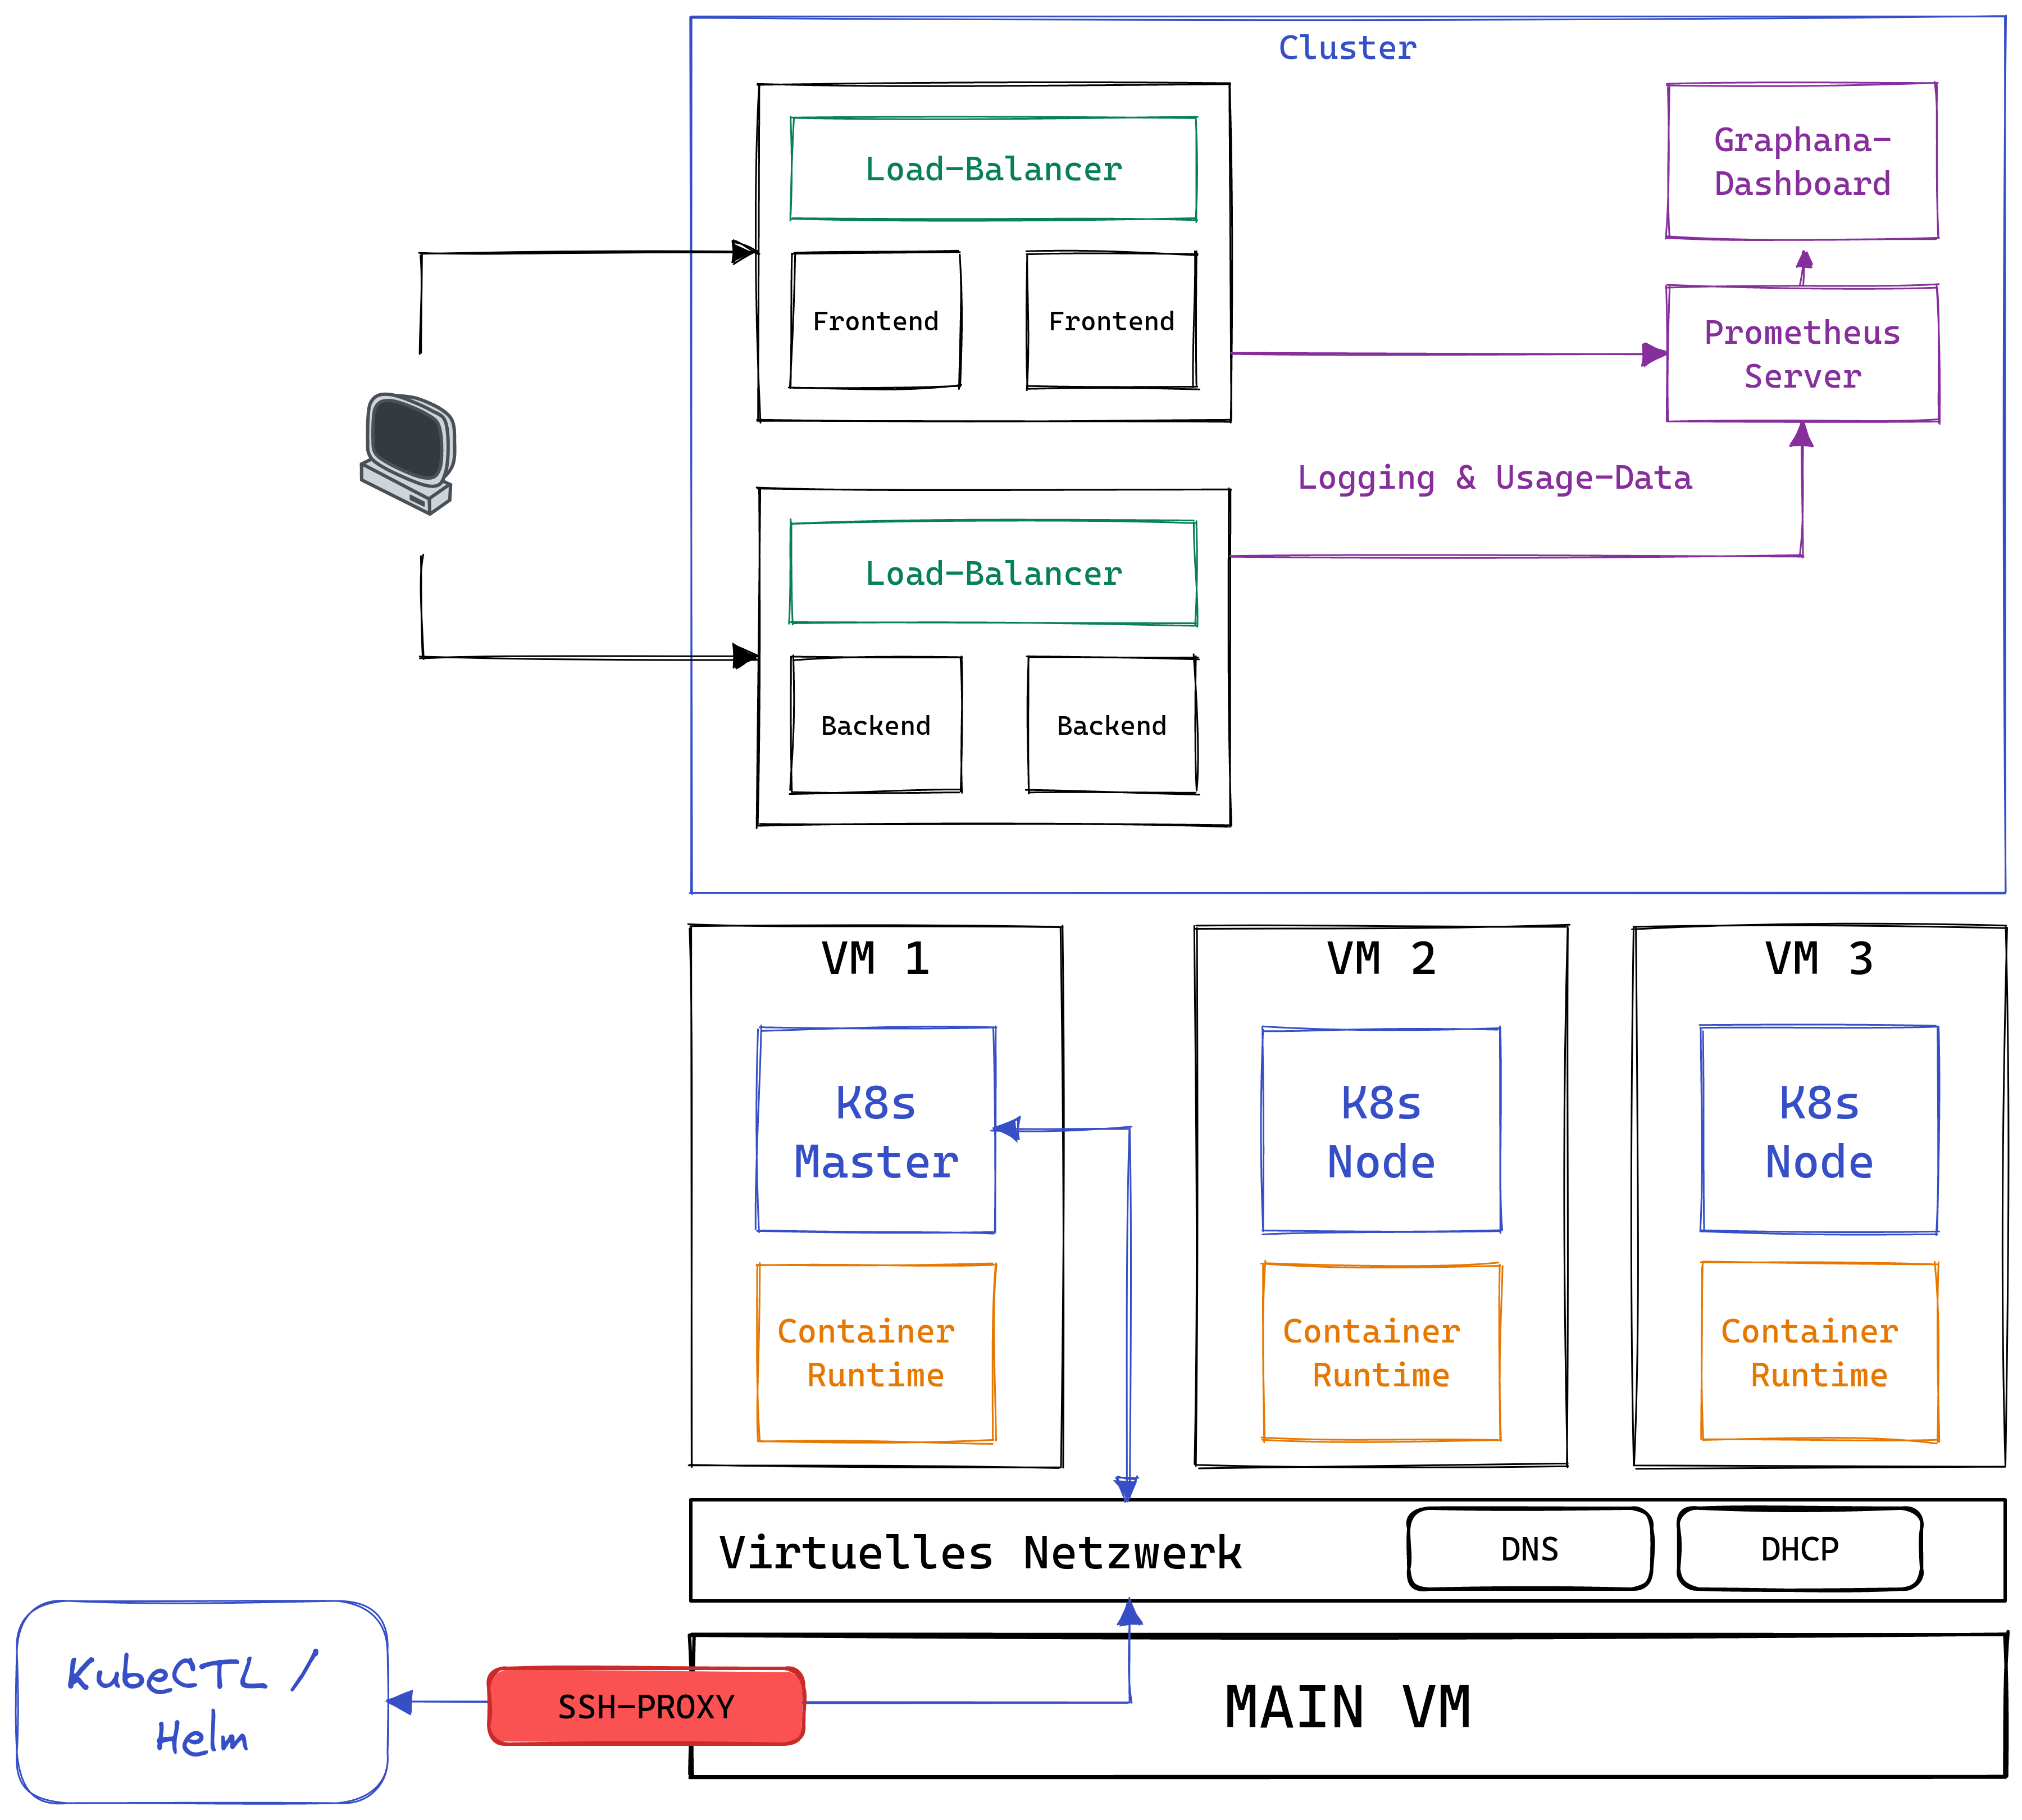
\includegraphics[width=15cm]{Bilder/architecture-overview.png}
        \centering
        \captionsetup{justification=centering, margin=1cm}
        \caption{Architecture concept for the service deployment with Kubernetes}
        \label{fig:Architecture}
    \end{figure}
\section{Setup}
    
\section{Usage}